\documentclass[utf8, 11pt]{feuille}

\newcommand{\titredutd}{\textbf{CC3 --- 2020}}

\begin{document}

\begin{center}
    \Large {\bf Contrôle continu}
    
    Lundi 30 novembre 2020 - durée: 2h00
\end{center}

Seules les calculatrices non communicantes et les notes manuscrites personnelles sont autorisées.

On rappelle les valeurs du nombre d'Avogadro ${\cal N_A}=6,02 \times 10^{23}$, de la constante de Boltzmann $k_B=1,38 \times 10^{-23}$ J.K$^{-1}$ et de leur produit, la constante des gaz parfaits $R=8,315$ J.K$^{-1}$.



% ______________________________________________________________________________
\section{Polarisation de spins atomiques}

Soit une substance dont les atomes sont magnétiques : ils possèdent un moment magnétique élémentaire (de spin) $\mu_0 \simeq 10^{-23}$ J.T$^{-1}$. A cause du caractère quantique du phénomène, la mesure de la projection de ce moment sur un axe ne peut prendre que deux valeurs $\pm \mu_0$. Pour polariser ces atomes (c'est-à-dire faire aligner leurs moments magnétiques) quand ils sont dans un gaz peu dense, on applique un fort champ magnétique $B$ et on refroidit à une température absolue $T$ suffisamment basse. Expliquer ces choix à la lumière de vos connaissances sur le facteur de Boltzmann. On pourra s'appuyer sur ce qui suit.
On produit couramment en laboratoire des champ magnétiques d'environ  5 T. \`A quelle température a-t-on trois fois plus de moments magnétiques parallèles au champ magnétique (supposé uniforme) que de moments magnétiques anti-parallèles au champ ? Il vous faudra exprimer le rapport entre la probabilité d'avoir un moment parallèle au champ et la probabilité d'avoir un moment anti-parallèle au champ en fonction de $\mu_0, k_B, B$ et $T$.



% ______________________________________________________________________________
\section{Système à trois niveaux}

On considère un système composé d'un grand nombre $N$ de molécules, dont les interactions sont négligeables, à l'équilibre avec un thermostat à la température $T$. Chacune des molécules possède quatre niveaux d'énergie \og interne \fg \, respectivement d'énergies -$\epsilon$, 0, 0 et  +$\epsilon$. On note $\beta=\frac{1}{k_B T}$. On rappelle les deux formules de trigonométrie hyperbolique : $\cosh(2u)=2 \cosh^2(u)-1$ et $\sinh(2u)=2 \sinh(u)\cosh(u)$.

\question
Quelle est la probabilité de trouver la molécule avec l'énergie -$\epsilon$ ? 0 ? +$\epsilon$ ? On pourra introduire $z(\beta)$ la fonction de partition d'une molécule.

\question
Montrer que l'énergie  moyenne $\overline{\epsilon}$ de la molécule est égale à $\overline{\epsilon}=- \epsilon \tanh ( \frac{\epsilon}{2k_BT})$. Quelle est l'énergie interne correspondante du système  ? Justifier votre réponse.

\question
En déduire la contribution $C$ de ces degrés de liberté énergétiques à la capacité calorifique \textbf{molaire} à volume constant de ce gaz.

\question
Tracer sommairement $C/R$ en fonction du paramètre $x=\frac{\epsilon}{2k_BT}$. Justifier pourquoi il y a forcément un maximum.

\question
Expliquer physiquement pourquoi ce maximum est obtenu pour $x \sim 1$. On pourra représenter sur un axe vertical les différents niveaux d'énergie et expliquer comment ils sont peuplés  dans les cas $k_BT \ll \epsilon$, $k_BT \sim \epsilon$ et $k_BT \gg \epsilon$.


% ______________________________________________________________________________
\section{Ultracentrifugation}

Un cylindre de révolution de rayon $R$, de hauteur $h$, d'axe $Oz$ contient $N$ molécules de masse $m$ d'un
gaz parfait en équilibre à la température $T$. On fait tourner ce cylindre autour de son axe
à la vitesse angulaire constante $\omega$. En régime permanent (lorsque le gaz a  été entraîné à la vitesse $\omega$ autour de $Oz$),  on admet qu'une molécule située à une distance $r$ de l'axe de rotation est soumise à une force centrifuge égale en module à $m\omega^2 r$.

\question
Comparer la force centrifuge au poids (à la surface de la Terre)  pour un rayon $r=20$ cm et pour une vitesse de rotation de 10 000 tours par minute.

\question
De quelle énergie potentielle $E_p(r)$ dérive cette force (attention au signe !) ?

\question
Calculer le quotient $\frac{p(r)}{p(0)}$ entre la probabilité $p(r)$ pour une particule d'être à la distance $r$ de l'axe et la probabilité $p(0)$ pour une particule d'être sur l'axe. Expliquer pourquoi ce quotient est aussi égal au rapport des densités particulaires  $\frac{n(r)}{n(0)}$. Application numérique avec les valeurs précédentes pour un gaz de masse molaire 352 g (de l'hexafluorure d'uranium) et à température ambiante. Commenter.

\question
Calculer l'expression de l'intégrale de configuration $Q_c$ associée à cette énergie, puis de l'énergie moyenne correspondante.



% ______________________________________________________________________________
\section{L'isotherme de Langmuir}

Le phénomène {\it d'adsorption} décrit le piégeage des molécules (de masse $m$) d'un gaz (à trois dimensions) sur la surface d'un solide (à deux dimensions) appelé substrat.  \`A l'équilibre thermodynamique, les molécules du gaz passent réversiblement de la phase gazeuse à la phase adsorbée.  Le nombre de molécules de la phase adsorbée n'étant pas constant, il est naturel d'utiliser le formalisme grand-canonique pour décrire cette phase 2D, dont le potentiel chimique est fixé par le gaz qui joue ici le rôle d'un grand réservoir. Soient $\rho$ la densité particulaire du gaz et $T$ sa température. On admet que le gaz est suffisamment dilué pour se comporter comme un gaz parfait. On note $h$ la constante de Planck.

\question
Rappeler l'expression du potentiel chimique $\mu$ du gaz en fonction de $\rho, k_B T$ et de la longueur d'onde thermique de de Broglie $\Lambda=\frac{h}{\sqrt{2\pi m k_B T}}$. En déduire que $\exp(\beta \mu)=\frac{P}{P_0(T)}$ où $P$ est la pression du gaz et $P_0(T)$ une fonction de la température seulement que l'on explicitera.

Dans le modèle de Langmuir les molécules adsorbées peuvent se fixer sur des sites réactionnels du substrat par une liaison chimique d'énergie $-\epsilon_0$.  Les $M$ sites du substrat sont discernables, indépendants et identiques et ne peuvent accueillir chacun au plus qu'une molécule.  On notera $n_i$ le nombre d'occupation du site $i$.  Le potentiel chimique des molécules de la phase adsorbée est égal $\mu$.

\question
Donner l'expression du nombre $N_a$ de molécules adsorbées et l'expression de l'énergie $E_a$ de la phase adsorbée en fonction des $\{n_i\}_{1\leq i \leq M}$ et de $\epsilon_0$.

\question
Calculer la grande fonction de partition $\Xi (T,M,\mu)$ de la phase adsorbée dans l'ensemble grand-canonique. On montrera qu'elle s'exprime comme $\Xi=\xi(T,\mu)^M$ où $\xi=1+e^{\beta(\mu+\epsilon_0)}$ est la grande fonction de partition d'un seul site.

\question
En déduire le nombre moyen $\langle N_a \rangle$ de molécules adsorbées ainsi que le taux de couverture de la surface $\theta=\frac{\langle N_a \rangle}{M}$  en fonction de $T$ et $\mu$. Montrer ensuite que
\begin{equation} \label{lang} 
  \displaystyle \theta(P,T)=   \displaystyle{\frac{P} {P+ P_0(T) {\rm e}^{-\beta \epsilon_0}}}
\end{equation}
Tracer l'allure de $\theta$ en fonction de la pression à température
fixée (courbe appelée isotherme de Langmuir).

\question
Les résultats d'une étude sur l'adsorption du trifluorométhane dans un zéolithe, sont présentés sur la figure \ref{FigLangmuir}. \'Evaluer $\epsilon_0$, l'énergie de liaison entre une
  molécule et le substrat.


\begin{center}
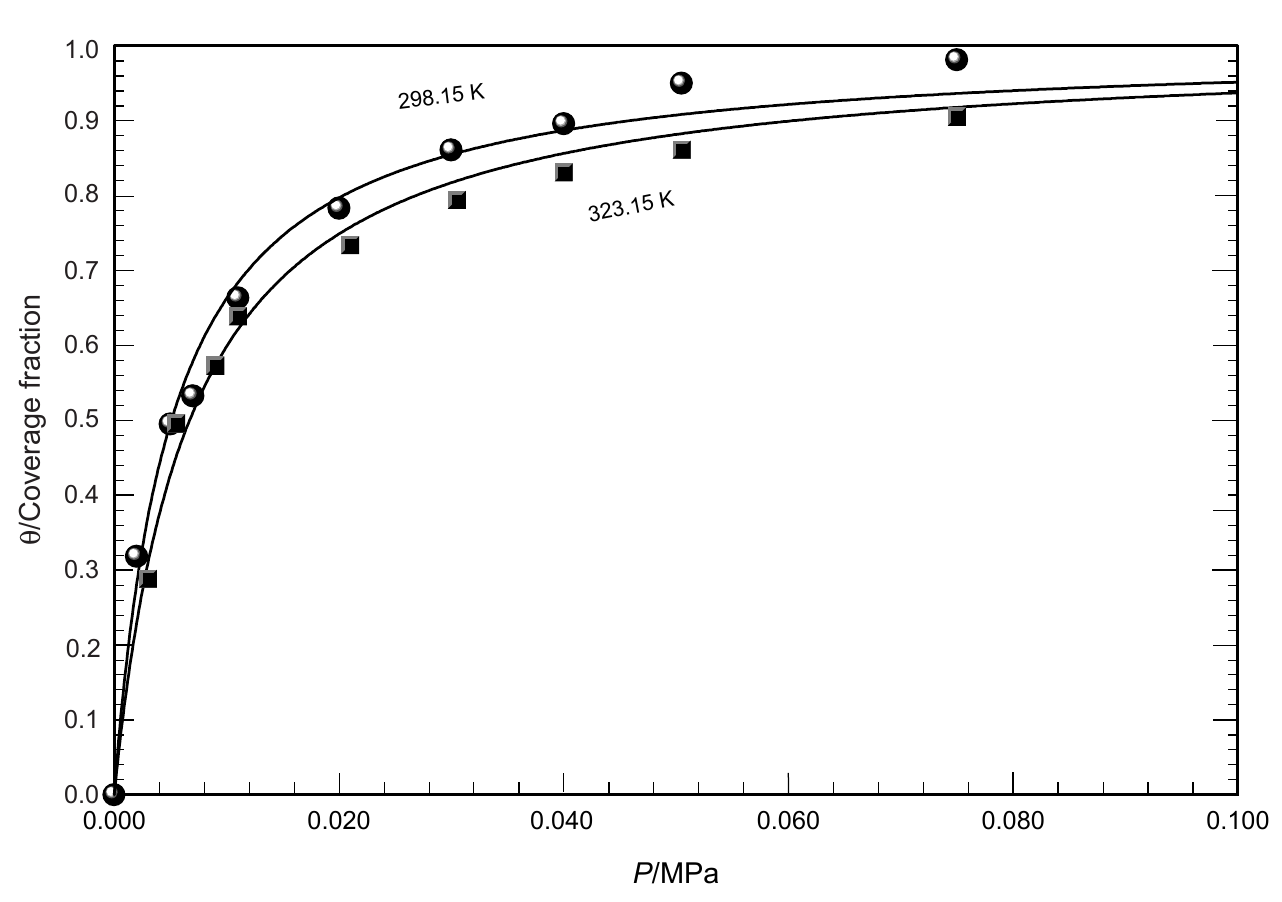
\includegraphics{Fig_Langmuir} \\
\textit{Taux d'adsorption $\theta(P)$  de CHF$_3$ en fonction de la pression $P$ (en MPa) à $T=298$ K et $T=323$ K dans une zéolithe. Les courbes représentent des isothermes de Langmuir données par l'équation (\ref{lang}) avec $P_0 \simeq 1,8$ bar (d'après M.B. Shiflett et al., Adsorption Science and Technology {\bf 31}, 59 (2013)). \label{FigLangmuir}}
\end{center}


\end{document}


